\documentclass[12pt]{report}

\usepackage{parskip}
\usepackage{adjustbox}
\usepackage{amstext}
\usepackage{amsmath}
\usepackage{graphics}
\usepackage{float}
\usepackage{hyperref}

\begin{document} 

\begin{titlepage}
\includegraphics[height=2.25cm,keepaspectratio]{lab.png}\hfill \includegraphics[height=2.25cm,width = 3.75cm]{pes.png}

\begin{center}
\vspace*{1cm}

\textbf{\Large{PES Innovation Lab}}

\vspace{0.3cm}
\text{\Large{Project Report}}
\vspace{0.1cm}
       
\text{\Large{Summer Internship 2022}}
       
\vspace{0.8cm}
\text{\huge{Vyaakaran}}
            
\vspace{0.8cm}
\text{\large{Interns}}
       
\vspace{0.2cm}
       
\begin{tabular}{c c}    
    \textbf{Name} & 
    \textbf{SRN} \\[0.5cm]
    \ {Tarun M} & {PES1UG20CS462} \\
    \ {Abishek Deivam} & {PES1UG20CS012} \\
    \ {Thejan N U} & {PES1UG20CS606} \\         
\end{tabular}
\vspace{0.5cm}

\text{\large{Mentors}}
\vspace{0.2cm}
       
\begin{tabular}{c c}
    \textbf{Name} & 
    \textbf{SRN} \\[0.5cm]
    \ {Akash Hamirwasia} & {PES2201800335} \\
    \ {Hrishit Chaudhuri} & {PES1UG19CS187} \\
\end{tabular}
       
\vfill
\vspace{0.5cm}
            
PES Innovation Lab\\
PES University\\
100 Feet Ring Road,\\
BSK III Stage,\\
Bangalore - 560085
            
\end{center}
\end{titlepage}


\begin{abstract}
Vyaakaran is an educational web-tool built to help anyone understand and visualize automata theory. It has support for Regular Grammar, Context Free Grammar and powerful testing tools to help the user test automata. We focus on extending this tool to enable simulation of a Turing Machine with it's tape. To be specific, we take state transitions from the user in a given syntax and pass it to a compiler to generate a graph and a tape to visualize the Turing Machine. 
\end{abstract}

\tableofcontents
%\listoffigures
%\listoftables

\chapter{Introduction}

\paragraph{What is Automata theory ?\\\\}
Theory of automata is a theoretical branch of computer science and mathematics. It is the study of abstract machines and the computation problems that can be solved using these machines.\\\\
Automata is a machine which takes some string as input and this input goes through a finite number of states and may enter in the final state or not. Any machine that converts information into different forms using a specific repeatable process is an automaton.\\

\paragraph{What is a turing machine ?\\\\}

A Turing Machine (TM) is a mathematical model which consists of an infinite length tape divided into cells on which input is given. It consists of a head which reads the input tape. A state register stores the state of the Turing machine. After reading an input symbol, it is replaced with another symbol, its internal state is changed, and it moves from one cell to the right or left. If the TM reaches the final state, the input string is accepted, otherwise rejected.\\\\
% Turing machines, first described by Alan Turing in Turing 1936–7, are simple abstract computational devices intended to help investigate the extent and limitations of what can be computed. Turing’s ‘automatic machines’, as he termed them in 1936, were specifically devised for the computing of real numbers. They were first named ‘Turing machines’ by Alonzo Church in a review of Turing’s paper (Church 1937). Today, they are considered to be one of the foundational models of computability and (theoretical) computer science.\\

\section{Problem Statement}
To create an environment to visualize and test Turing Machines.\\
User gives instructions and then Vyaakaran simulates how a Turing Machine
would run it.
% How would the user specify instructions?
% ○ As a set of state transitions. (There are some tools that do this)
\paragraph{Why this problem ?\\\\}
We chose this problem as automata theory is not an easy subject to understand , primarily because there are not a lot of tools built around it. The existing tools are primitive and are harder to get started with for complete beginners.
\\\\
The rest of our report will go on about how we approached the problem and went about solving it.
% You can conclude the introduction by writing how the rest of the report is organised.

\chapter{Literature Survey/Related Work} 
% Length: [1-3 pages]. 
% Are there existing solutions to your problem? If yes, elaborate in a few lines. You can also write about the theory/concepts associated with your project. Cite related work  \cite{wiki:latex}.  You can conclude this section by stating how your work is novel/different from the related work you have just described. For each paper or link that you mention here, please include a short summary of the resource as well as how the resource contributed to your project.

There are a few tools available online similar to Vyaakaran:\\
\begin{itemize}
\item CFG Developer - web.stanford.edu/class/archive/cs/cs103/cs103.1156/tools/cfg/\\
\item Turing Machine simulator -  turingmachinesimulator.com\\
\end{itemize}

But none of them come close to the feature set and unified experience
Vyaakaran provides right now.

Our initial approach was to have the user input as unrestricted grammar and construct the turing machine from it. However on further research we found that this was not possible as no solid conversion exists. At best we were able to only build a turing machine unique to the input string that accepts only that string .Even this turing machine was possible only if the computer was able to determine in a 'non deterministic' manner which transitions to accept and which to ignore
hence we changed our approach to have the user input state transitions and generate the turing machine from that.
\cite{wiki:tm1}
\cite{wiki:tm2}
\cite{wiki:tm3}
\cite{wiki:tm4}
\cite{wiki:tm5}

\chapter{Main Body}

The simulator needs an input from the user in a specified format , then converts that input into a parse tree , then a graph and displays it as an interactive tape and as a state transition diagram

\section{User Input}
We had to design a user friendly syntax that was both easy to learn and understand
\begin{align*}
 &S \; ( \;a \;: \;x \;) \;-\!>\!- \;Q1 \\
 &Q1 \;(\; b\; :\; y \;)\; -\!<\!- \;Q2 \\
 &Q2 \;(\; c \;: \;z \;) \; -\!=\!- \; *Q3 
\end{align*}

We decided upon the above syntax for user input as it seemed simple enough for the user to input and understand with some simple rules -\\
S represents the start state \\
*Statename represents the final state\\
$ >,<,= $ represents the movement direction of the tape ie right , left , stay \\
so the first line essentially translates to \\ 
from start state 'S' read a symbol 'a' replace it with 'x' , move 'right' on the tape and go to next state 'Q1'\\
State names begin with capitals letters , while symbols begin with lowercase letters

\section{Compiler}
The Vyaakaran compiler is used to break down the user's program into a parse tree and then into a graph which is easier to display in the webtool.

\subsection{Lexical Analyser}
The first phase of our compiler is the lexer (lexical analyser). The lexer reads the stream of characters making up the user's input and groups the characters into meaningful sequences called lexemes. For each lexeme, the lexer produces a token which has information like token-name and token-value which will be used by the parser. The lexer we built has various tokens for different types of input we need to handle. The tokens used are listed below:
\begin{itemize}
    \item StartState:   The character 'S', starting state of a TM
    \item State:        Represents a state in a TM
    \item FinalState:   The TM accepts the string
    \item Symbol:       Any character on the input tape of the TM
    \item LParen:       A left parenthesis '('
    \item RParen:       A right parenthesis ')'
    \item Colon:        A colon used as a seperator ':'
    \item Hyphen:       Used along with Dir as a seperator
    \item Dir:          Provides the direction the tape head moves in
    \item Whitespace:   Skipped by the lexer
    \item NewLine:      Denotes the end of a line and start of a new line
    \item Comment: Comments in a programming language
\end{itemize}
\subsubsection{Errors}
The lexer raises an error if any unidentified tokens are found in the input.
\begin{figure}[H]
  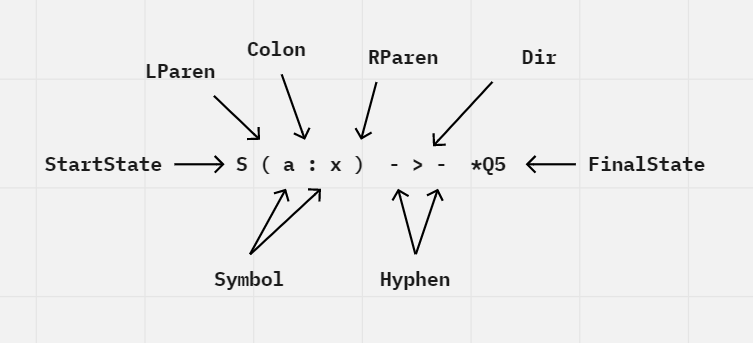
\includegraphics[width=\columnwidth]{lexerSample.png}
  \caption{Sample Tokens}
\end{figure}

\subsection{Parser}
The second phase of the compiler is syntax analysis or parsing. The parser uses the first components of the tokens produced by the lexical analyzer to create a tree-like intermediate representation that depicts the grammatical structure of the token stream which is called the parse tree. Here is our parse tree's grammar.
\begin{align*}
&START \; -> State \; Replacement \; Move \;  State \; ?  \; ( NewLine \; START ) \\
&Replacement \; ->  LParen \; Symbol \; Colon \; Symbol \; RParen \\
&Move \; -> Hyphen \; Dir \; Hyphen
\end{align*}
\subsubsection{Errors}
The parser raises errors if the tokens are not according to the grammar expected by it. This rejects input that might be a random combination of tokens which have no meaning as such.

\subsection{Semantic Analyser}
The semantic analyser uses the parse tree and the token list to validate if the user input in semantically consistent with our language definition i.e. our grammar
\subsubsection{Graph}
With the given parse tree a graph of the Turing Machine is generated. This is both used for display in the frontend and for performing graph checks in the backend. The graph checks are:
\begin{itemize}
    \item A state is both used as a final state and a non-final state.
    \item Final state is reacheable from the Start state.
    \item A Turing Machine needs to have a Start State and a single Final State.
    \item Two edges from a state have the same Read Symbol.
\end{itemize}
% This is the heart of your report. It describes your project. It can be more than one chapter/section. For example : 'System model', 'methodology', 'solution method', 'approach'. Include diagrams, flow charts, algorithms etc. if relevant. Make sure you refer to all figures and tables that you include in the text. Like this: In Figure \ref{solvay}, the IQ level is over 9000! (Read in Vegeta voice.)
%template for figure

\begin{figure}[h!]
  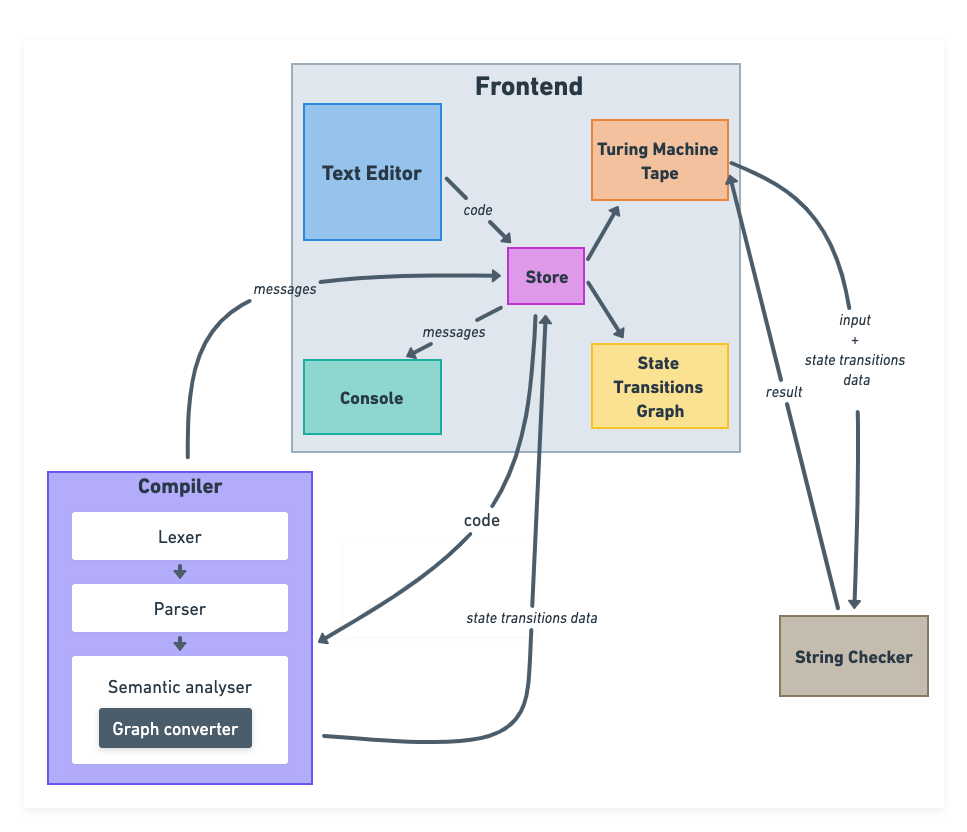
\includegraphics[width =\columnwidth ]{workflow.png}
  \caption{Workflow Diagram}
\end{figure}

\section{Hardware and Software Requirements}
% What hardware/software did you use? Can be lists or tables if you used many. Mention version numbers of software. Mention stats. of the computer you did your project on. \\
The client side requirement is a JavaScript-enabled browser. The compiler is built with typescript and a parser building toolkit called chevrotain. The website and editor are built with Vue, SvelteKit and monaco editor (powers VS Code).
% \section{Artifacts}
% What are the Inputs that your system requires? In an Ideal Scenario, what are the outputs? How do certain inputs impact the output, if there exists such a mapping? Do add in a workflow diagram of the system to ease explanation and improve understanding.


\chapter{Results and Discussion}
At this stage Vyaakaran currently supports Regular Grammar, Context Free Grammar and Turing Machine simulations. It can be accessed by anyone on \href{https://vyaakaran.vercel.app/}{vyaakaran}\\

 
\begin{figure}[H]
\centering
  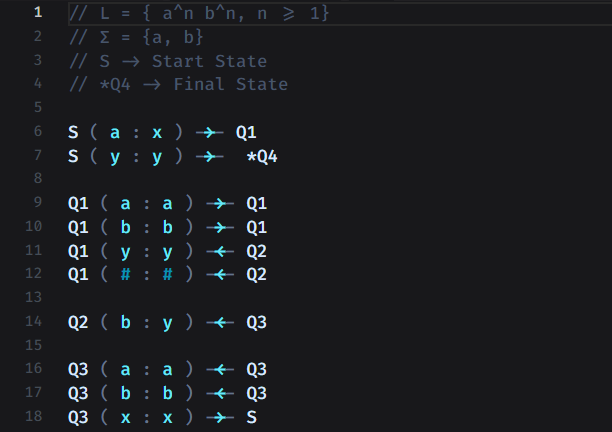
\includegraphics[scale=0.8 ]{inputOutput.png}
  \caption{The input given by the user}
\end{figure}


\begin{figure}[H]
  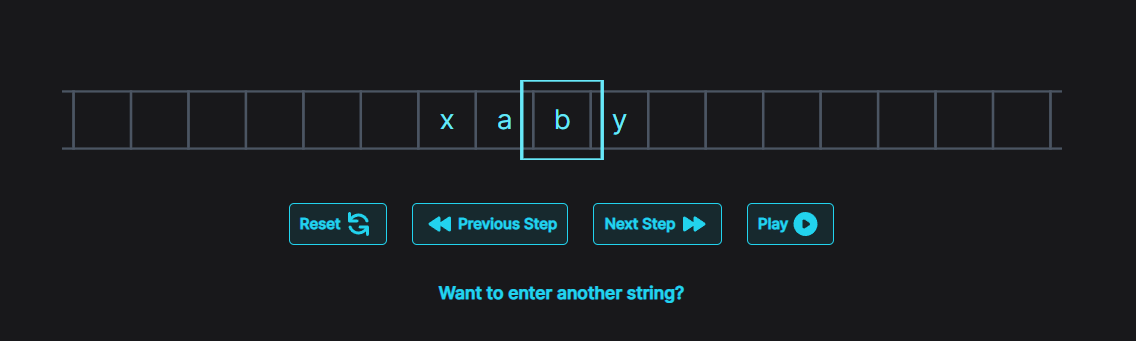
\includegraphics[width=\columnwidth ]{tapeOutput.png}
  \caption{The interactive tape that the turing machine takes input from and performs operations on. The user can view a step by step process of how the turing machine accepts a string.}
\end{figure}

\begin{figure}[H]
  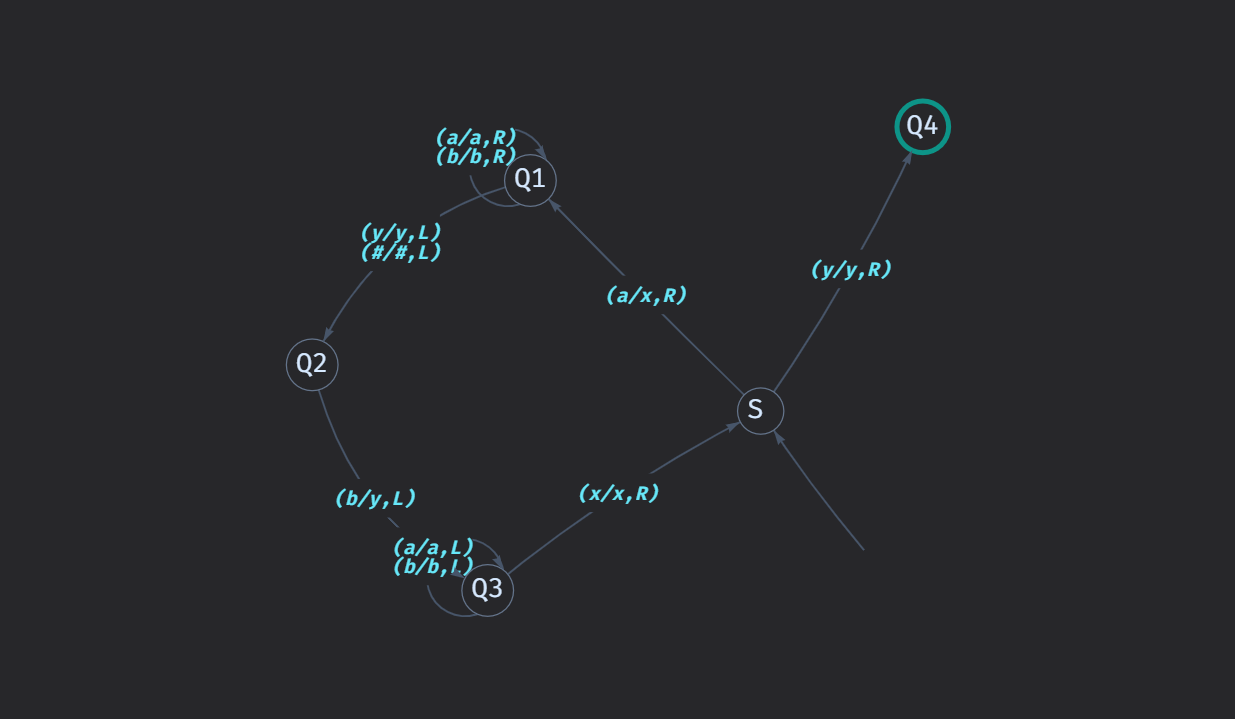
\includegraphics[width=\columnwidth ]{graphOutput.png}
  \caption{The state transition diagram that represents the turing machine in a simple format of states and transitions}
\end{figure}



\begin{figure}[H]
  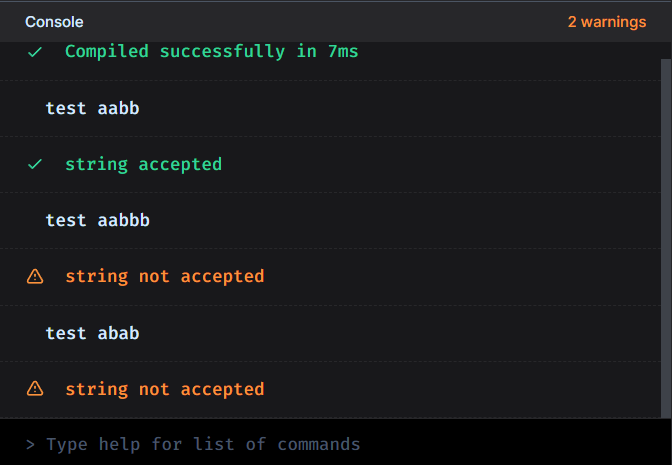
\includegraphics[width=\columnwidth ]{consoleOutput.png}
  \caption{The console which has basic commands to compile , clear , and test strings. The compile command compiles the user input, the clear command clears the console, the test command is used to test strings through the turing machine defined by the user without the hassle of using the tape display to see whether the turning machine accepts the string.}
\end{figure}



\chapter{Conclusions and Future Work}
There is always scope for future improvement, with plans for adding more features and functionalities. Vyakaraan right now is still a very useful tool for anyone interested in learning automata theory, and our contribution of the turing machine simulator is a easy to use feature, with the user giving in instructions and getting the tape along with its features and state transition diagram as an output. \\
The turing machine simulator can further be improved by taking the user input as a pseudo code which is a much simpler way of entering instructions.

%Please make sure you keep a log of all the resources you have used. This includes websites, tutorials, videos, papers or even blogs can be cited.

\bibliographystyle{ieeetr} 
\bibliography{bibmil.bib}
\appendix 
\chapter{Website and repository}
website :
\href{https://vyaakaran.vercel.app/}{vyaakaran}\\\\
repository : 
\href{https://github.com/blenderskool/vyaakaran}{github}
\end{document}
